\subsection{Normalisation and error bars} \label{sec:errorbars}
The transmissions graphs in the results section are normalised. In the graphs in Fig. \ref{fig:transmissionkilde2conc} (multimeter), each data point has an error bar. Likewise, each data point in Fig. \ref{fig:transmissionkilde3} (supercontinuum) has an error bar. In addition, the error bars in Fig. \ref{fig:transmissionkilde3} are connected for easier readability. We normalised and obtained these error bars in the following way:

\begin{itemize}
    \item The spectrum of a reference waveguide consists of $N$ data points with transmission values $x_{r}$. See Appendix for reference spectra.
    \item The spectrum of a structure as outlined in the "Experimental setup" section, consists of $N$ data points with transmission values $x_{m}$.
    \item The data is normalised by $x_n = x_{m} - x_{r}$. Usually one would divide the measurements, $ x_n = \left( \frac{x_{m}}{x_{r}} \right)$, but the readings have a unit dBm which is derived from $\log_{10}$. $\log \left({\frac{a}{b}} \right) = \log{a} - \log{b}$. When subtracting, the normalised transmissions are left with the preferred unit dB.
    \item The data points (usually $N$ = 1000) were grouped in blocks of 5. 
    \item For each block, the average $\bar{x_n}$ was computed and used as the middle point.
    \item The minimum $x_n$-value in each block is the lower end of the error bar, the maximum $x_n$-value in each block is the upper end of the error bar.
\end{itemize}

The rationale for this method of computing uncertainties is that the transmission as a function of wavelength is expected to be a smooth curve. 5 consecutive data points should be near each other, assuming the reading is based on many samples, i.e. the method is valid for large values of $N$.\\
\\
This method has a weak spot: It cannot determine whether the experimental results can be reproduced. To counter this, we performed a series of test (see the "Statistics" section) to check reproducibility.

\subsection{Broadband light source}
The measurements on our silicon structures resulted in some challenges. The first set of measurements were performed with a broadband light source. The data for our 6 structures all had an ongoing problem; the signal was too noisy, see an example in Fig. \ref{fig:Lightsource1Rep} for box 40 nm.

\begin{figure}[H]
    \centering
    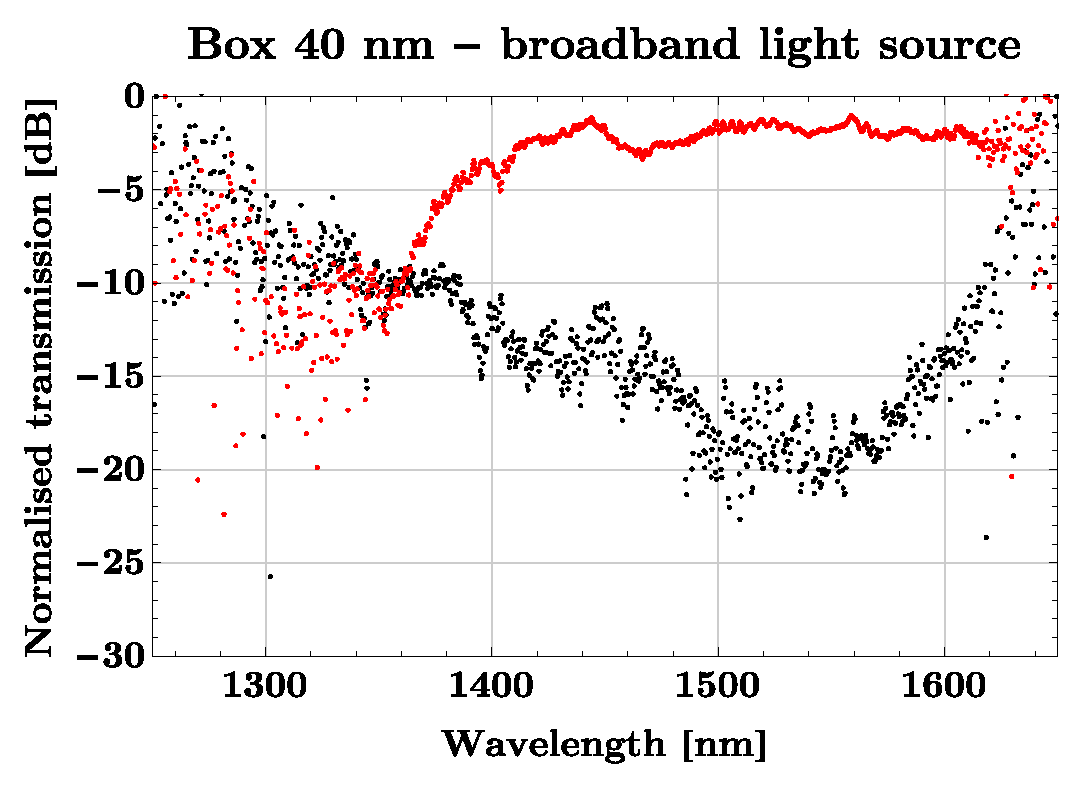
\includegraphics[width=0.6\textwidth]
        {fig/Kilde1Broadband/box40broadband.pdf}
    \caption{Data from box structure w. minimum feature size of 40 nm from a broadband light source. Black: Signal through upper output waveguide. Red: signal through lower output waveguide. This graph has no error bars, but all conclusions regarding the fabricated designs were based on data obtained by other light sources. The broadband light source yielded too noisy data, as seen on the plot.}
    \label{fig:Lightsource1Rep}
\end{figure}

As shown in the right side of Fig. \ref{fig:Lightsource1Rep}, the signal around 1550 nm in the lower output waveguide was significantly clearer, which can be explained by the intensity profile of the LED emitting more light with wavelength around 1500 nm. The structure is designed to split light into 1300 nm and 1550 nm. 

Because of too much noise, especially in the low wavelength range, it is difficult to draw a conclusion from the data.

The 1300 nm wavelength is too far from the 1430 nm peak wavelength that the LED produces, which means that the data obtained primarily is background noise.

\subsection{Multimeter light source}

The multimeter had 2 LEDs with peak wavelengths at 1310 nm and 1550 nm, respectively. Because the individual bandwidths of the light sources were too narrow to cover the wanted spectrum, we gathered data using both light sources and concatenated the data from the useful (non-noisy) regions to get a full wavelength spectrum. Specifically, the data points from 1200 nm to 1400 nm were measured with the light source peaking at 1310 nm. The data points from 1400 nm to 1650 nm were measured with the light source peaking at 1550 nm. The results are plotted in Fig. \ref{fig:transmissionkilde2conc}.

This method yielded more useful results than with the broadband LED. Even so, some of the data is still very noisy, which is why we have also measured using the supercontinuum light source.

\subsection{Supercontinuum light source}
The supercontinuum light source yielded significantly clearer results, as seen in Fig. \ref{fig:transmissionkilde3}. That said, the results are very comparable to the multimeter results from Fig. \ref{fig:transmissionkilde2conc}. 


